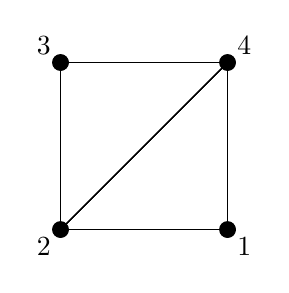
\begin{tikzpicture}
\def \n {1}
\def \R {1.5cm}
\def \RR {1.8cm}
\draw (-45:\R) \foreach \x in {-135,-225,-315} {
            -- (\x:\R)
        } -- cycle;
\foreach \x in {-45,-135,-225,-315} {
        \draw [fill] (\x:\R)  circle [radius=0.1];
        }
\foreach \x/\i in {-45/1,-135/2,-225/3,-315/4} {
        \node at (\x:\RR) {\i};
\draw (-135:\R) -- (-315:\R);
        }
\end{tikzpicture}
